\documentclass[12pt, twoside]{article}
\usepackage[francais]{babel}
\usepackage[T1]{fontenc}
\usepackage[latin1]{inputenc}
\usepackage[left=1cm, right=1cm, top=8mm, bottom=8mm]{geometry}
\usepackage{float}
\usepackage{graphicx}
\usepackage{array}
\usepackage{multirow}
\usepackage{amsmath,amssymb,mathrsfs}
\usepackage{textcomp}
\pagestyle{empty}
\usepackage{soul}
\begin{document} 

NOM: \\
PRENOM:  

\medskip


\begin{center}
{\fbox{$2^{de}5$ \qquad \qquad \textbf{\Large{Devoir surveill� 6}}
\qquad \qquad 20/03/2009}}
\end{center}


\bigskip


\textbf{Exercice 1:} \textit{(4.5 points)}

La figure ci-dessous montre la courbe repr�sentative $\mathcal{C}_{f}$ d'une
fonction $f$ d�finie sur l'intervalle $[-15;1]$. Les 6 points en gras
appartiennent � $\mathcal{C}_{f}$.  

\enskip

\begin{center}
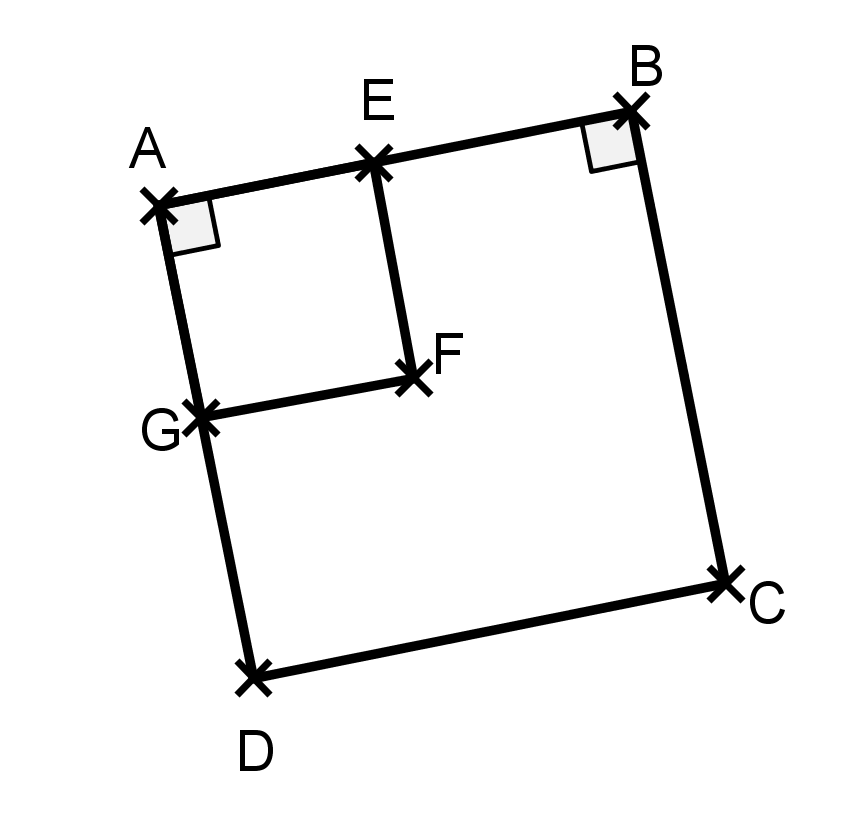
\includegraphics[width=13cm]{images/ex1.png} 
\end{center}


A l'aide de ce graphique, d�terminer parmi les affirmations ci-dessous: celles
qui sont vraies (V), celles qui sont fausses (F), celles pour lesquelles le
graphique ne permet pas de r�pondre (P).

\enskip

\textit{\ul{Remarques}: Chaque r�ponse exacte rapporte 0.75 point; une
r�ponse inexacte enl�ve 0,25 points; une question ne rapporte ni n'enl�ve aucun point. Si le
total est n�gatif, il est ramen� � z�ro.}

\enskip
 
\begin{tabular}{|c|m{14cm}|c|c|c|}
\hline
1 &  Les images de $0$ sont: $-5$, $-1$ et $1$ & V & F & P \\
\hline
2 & Sur l'intervalle $[-15;1]$, le nombre $2$ a deux ant�c�dents par la
fonction $f$ & V & F & P \\
\hline
3 & $f(x)\leqslant 0$ pour $x \ \in [-15;-5] \cup [-1;1]$ & V & F &P \\
\hline
4 & Sur l'intervalle $[-15;1]$, l'�quation $f(x)=-5$ admet deux solutions & V &
F & P \\
\hline 
5 & $f(-3,568)>f(0,71)$ & V & F & P \\
\hline
6 & Sur l'intervalle $[-15;1]$, l'in�quation $f(x) \geqslant -15$ n'a pas de
solutions & V & F & P \\
\hline
\end{tabular}


\bigskip

\bigskip

\bigskip

\textbf{Exercice 2:} \textit{(5 points)}

$A$, $B$, $C$ et $D$ sont quatre points d'un cercle. On
note $I$ le point d'intersection des droites $(AC)$ et $(BD)$. 

\enskip

\begin{tabular}{cc}
\begin{minipage}{13cm}
\begin{enumerate}
  \item Donner la d�finition de deux triangles semblables.
  \item D�montrer que les triangles $AIB$ et $DIC$ sont semblables.
  \item Ecrire les sommets homologues. En d�duire les �galit�s de rapports.
  \item On suppose que $AB=20cm$, $DC=10cm$, $ID=8cm$ et $IC=5cm$ (la figure
  n'est pas � l'�chelle).
  \begin{enumerate}
    \item Calculer $AI$ et $IB$.
  \item Calculer le rapport des aires des triangles $AIB$ et $CID$.
  \end{enumerate}
  \end{enumerate}
\end{minipage}
&
\begin{minipage}{5cm}
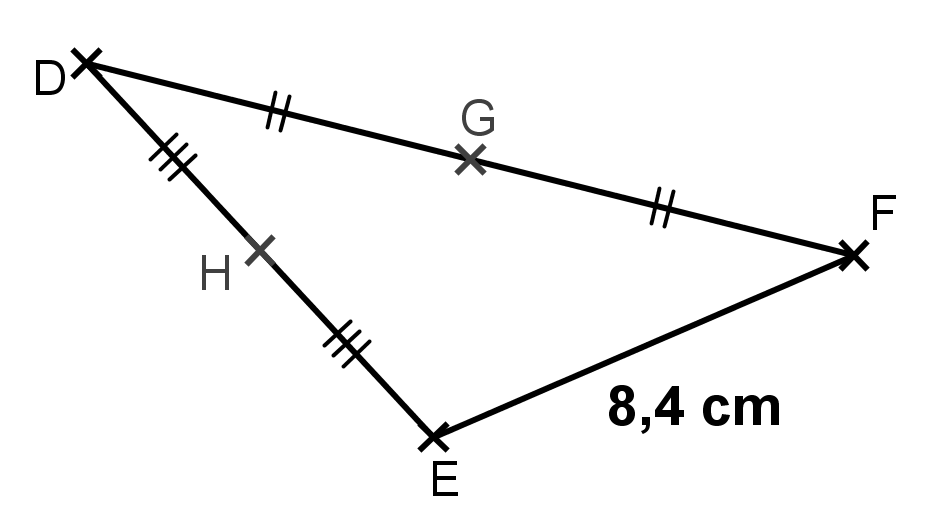
\includegraphics[width=5cm]{images/ex2.png}
\end{minipage}
\end{tabular}

\pagebreak

NOM: \\
PRENOM: 

\bigskip

\textbf{Exercice 3:} \textit{(4 points)}

\begin{tabular}{cc}
\begin{minipage}{14cm}
Sur la figure ci-contre, $OCD$ et $OAB$ sont des triangles
�quilat�raux et $OCEB$ est un rectangle.
\begin{enumerate}
  \item D�montrer que les triangles $ABE$, $ECD$ et $AOD$ sont isom�triques.
  \item En d�duire la nature du triangle $AED$.
\end{enumerate}
\end{minipage}
&
\begin{minipage}{4cm}
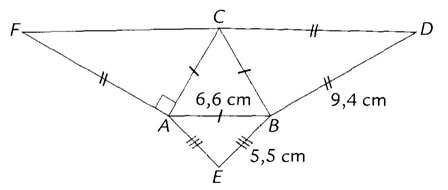
\includegraphics[width=4cm]{images/ex3.png}
\end{minipage}
\end{tabular}

\bigskip

\textbf{Exercice 4:} \textit{(6.5 points + 1 bonus)} 

\enskip

\textit{\ul{Remarques}: Il est fortement conseill�
de faire des sch�mas en plus de la figure. La construction de la figure sera
compt�e dans le bar�me, elle peut se faire m�me si les questions ne sont pas
trait�es.}

\enskip

Deux cercles $\mathcal{C}$ et $\mathcal{C}'$ (de centres
respectifs $O$ et $O'$ et de rayons respectifs $r$ et $r'$) se coupent en deux
points $A$ et $B$. On trace le diam�tre $[AE]$ de $\mathcal{C}$ et le diam�tre
$[AF]$ de $\mathcal{C}'$.

\begin{enumerate}
  \item Compl�ter la figure ci-dessous.
  
  \bigskip
  
  \bigskip
  
  \bigskip 
  
  \bigskip
  
  \bigskip
  
  \bigskip
  
  \bigskip
  
  \bigskip
  
  \bigskip
  
  \bigskip
  
  \begin{center}
 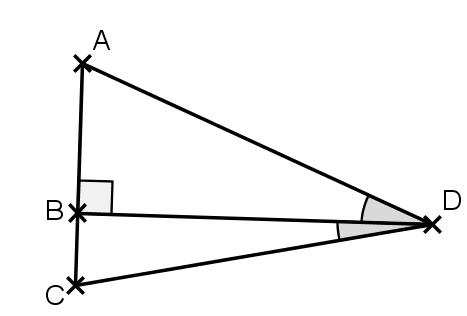
\includegraphics[width=9cm]{images/ex4.png} 
 \end{center}

 \item Que peut-on dire des triangles $AEB$ et $ABF$? En d�duire que les points
 $E$, $B$ et $F$ sont align�s.
 \item La droite $(AE)$ coupe le cercle $\mathcal{C}'$ en $P$. La droite $(AF)$
 coupe le cercle $\mathcal{C}$ en $Q$.
 
 \begin{enumerate}
   \item D�montrer que les triangles $EQA$ et $FPA$ sont semblables.
   \item En d�duire que $AQ \times FA=AP \times EA$.
   \item D�terminer en fonction de $r$ et $r'$ le rapport de l'aire de $EQA$ �
   celle de $FPA$.
  
 \end{enumerate}
 
 \item Les droites $(PF)$ et $(QE)$ se coupent au point $I$.
 
 \ul{BONUS}: Montrer que la droite $(AB)$ passe par $I$.
 \item Montrer que les triangles $IPE$, $EQA$, $IQF$ et $FPA$ sont semblables. 
\end{enumerate}

\end{document}
